\section{Objekterkennung}

Abbildung \ref{fig:1} zeigt die Ausgangslage.

Das   Bild   wird   als  erstes  in   den   HSV-Farbraum   transformiert   und
tiefpass-gefiltert,   um   das   Rauschen   ein   bisschen   entgegenzuwirken.

\begin{figure}[H]
    \centering
    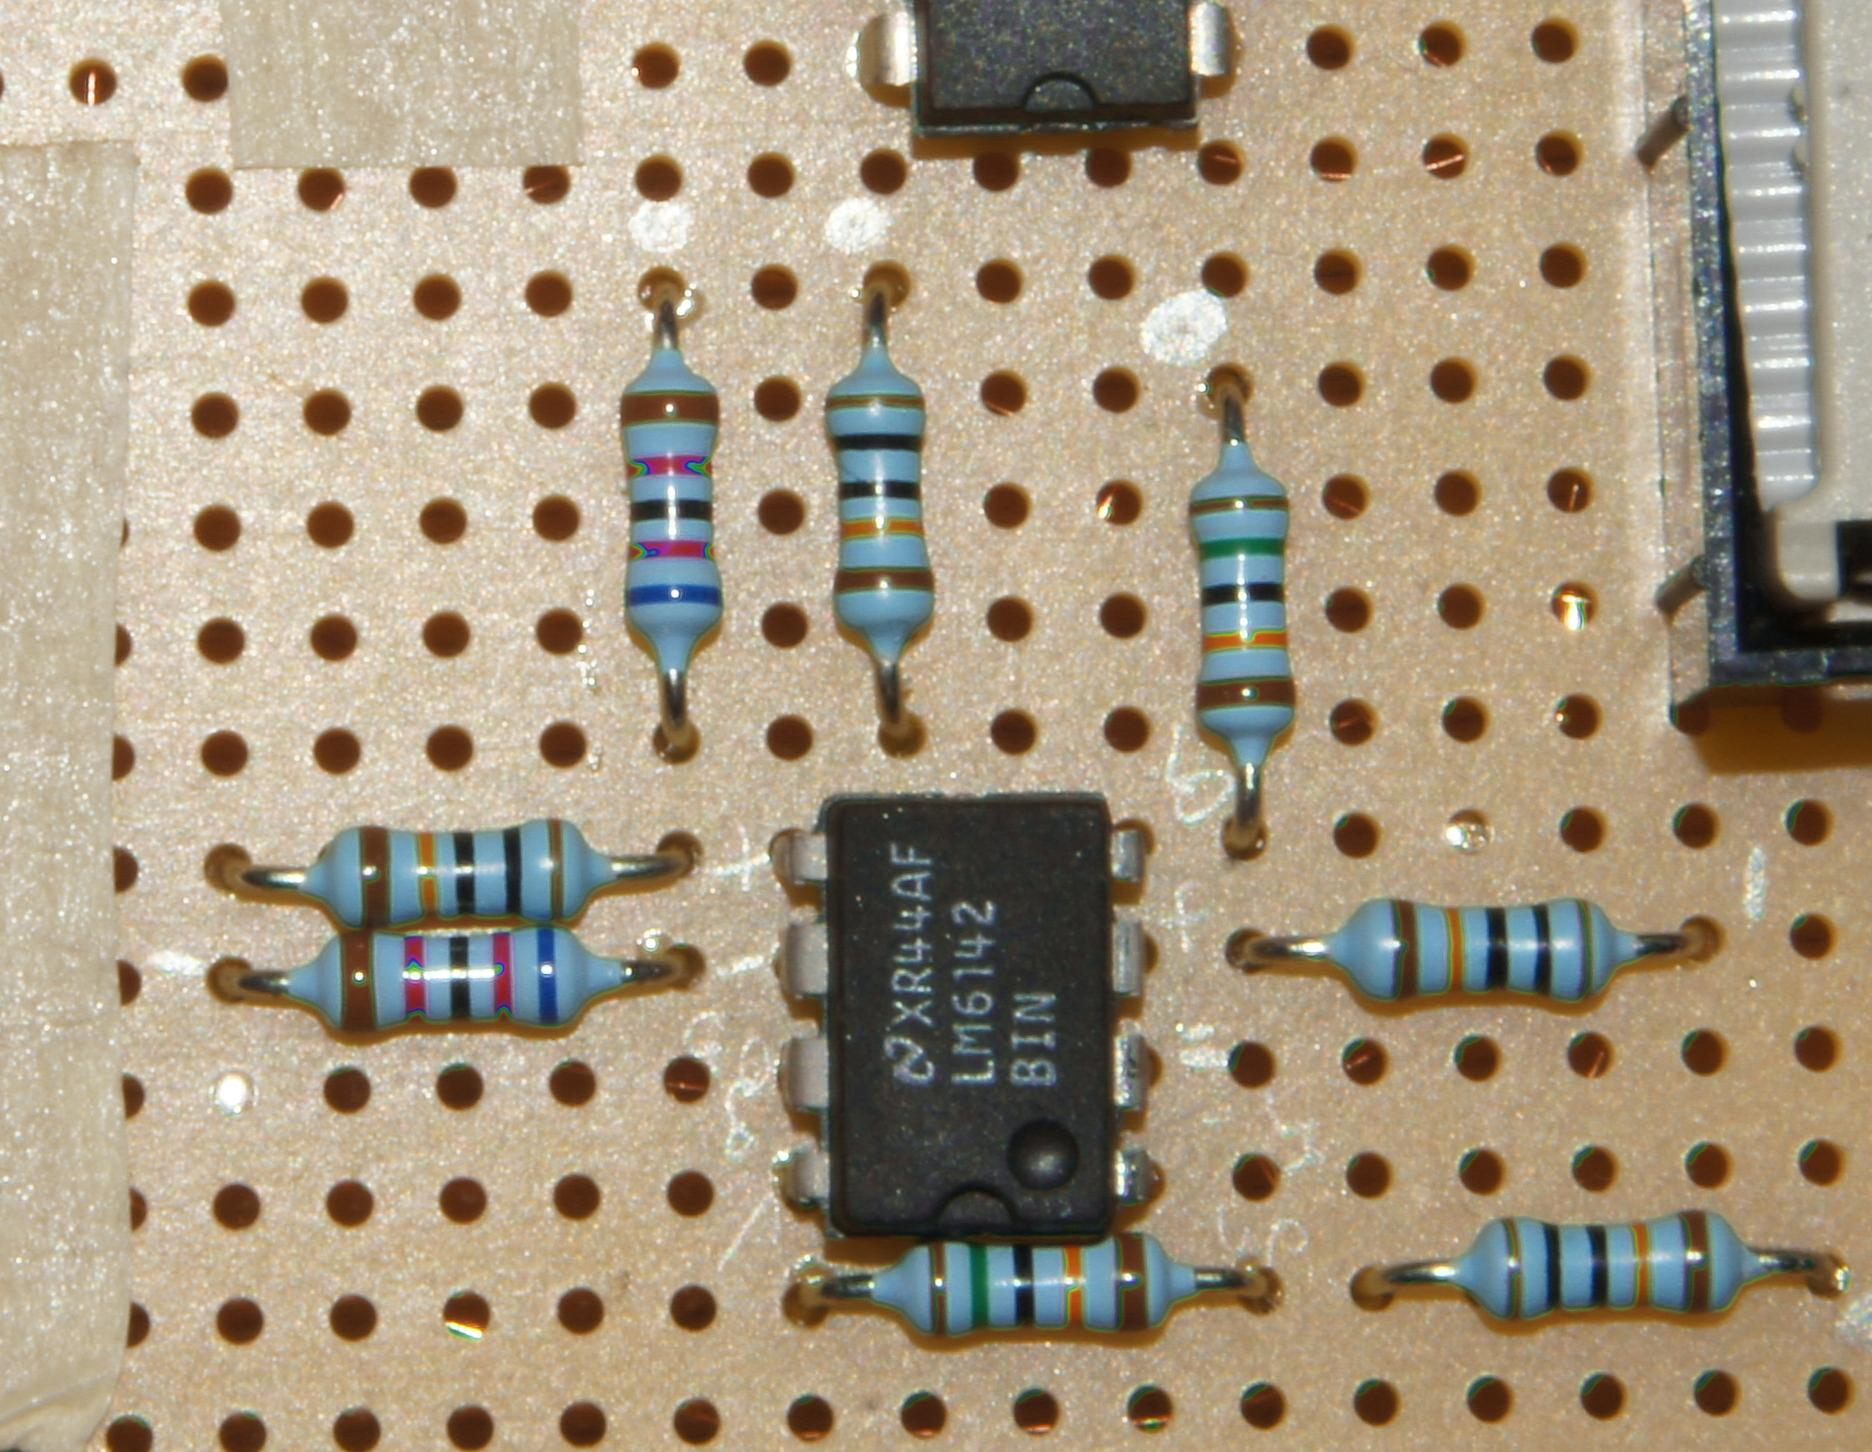
\includegraphics[width=.7\linewidth]{images/1}
    \caption{Ausgangslage}
    \label{fig:1}
\end{figure}

Die  blaue  Farbe  der  Widerst\"ande wird ausgenutzt, um die Widerst\"ande zu
isolieren. Eine  Maske  wird generieriert (siehe Abbildung \ref{fig:3}) welche
nur die blauen Teile des Bildes enth\"ullt. Die Vorgehensweise daf\"ur ist ein
einfaches Thresholding im HSV-Farbraum.

Diese  Maske  enth\"alt  noch  viele  Artefakte  die  mittels  eines  Openings
gr\"osstenteils  entfernt  werden  k\"onnen.  Ein Nachteil hier ist  dass  die
Filtergr\"osse  von der Widerstandsgr\"osse  abh\"angt,  aber  wir  zu  diesem
Zeitpunkt  nicht  wissen  k\"onnen,  wie  viele Pixel ein Widerstand  im  Bild
besetzt.  F\"ur  die  Bilder, die wir verwendet haben, benutzten wir  ein  4x4
Filter.

\begin{figure}[H]
    \centering
    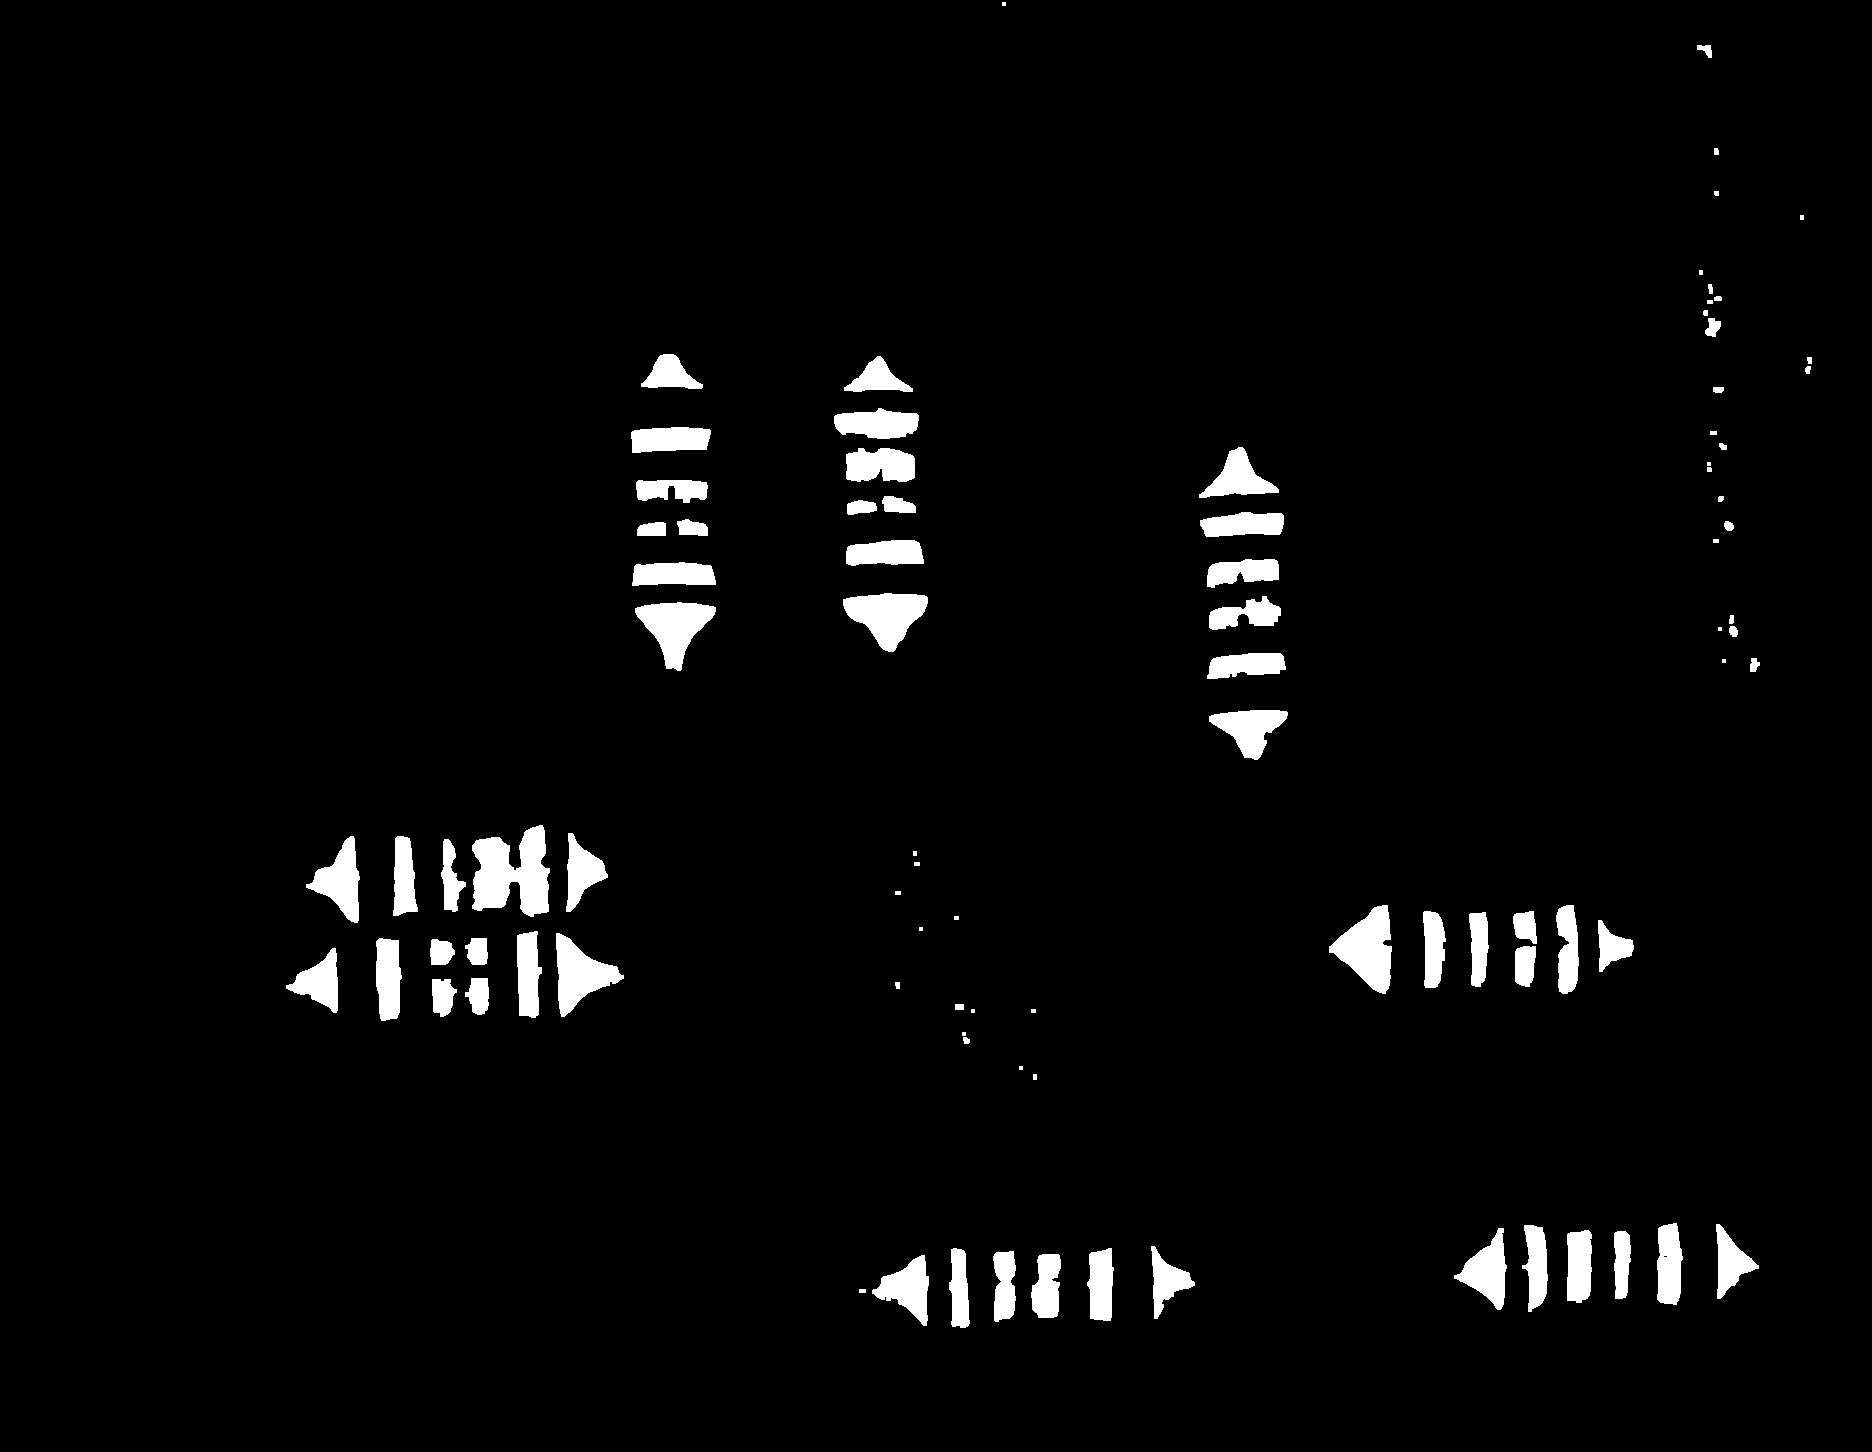
\includegraphics[width=.7\linewidth]{images/3}
    \caption{Maske, nach Blau gefiltert}
    \label{fig:3}
\end{figure}

Als  n\"achstes  wird  eine   Partikelanalyse   durchgef\"uhrt.  Vorallem  von
Interesse  ist  die  umh\"ullende  Ellipse  der   Objekte,   weil  daraus  die
Orientierung und die H\"ohen- und Breitenverh\"altnisse der Objekte analysiert
werden  kann.  Wie  in  Abbildung  \ref{fig:4}  demonstriert  wird,  wird  die
Geometrie der  Ringe (oder genauer: Die Geometrie des Zwischenraums der Ringe)
ausgenutzt.

Partikel, die mehr als  $2.5$  mal  so  hoch  sind  wie  Breit  (in  Abbildung
\ref{fig:4} als Rot  markiert) werden behalten. Partikel, die dieses Kriterium
nicht  erf\"ullen  (in  Abbildung  \ref{fig:4}  als  Blau  markiert),   werden
eliminiert.

\begin{figure}[H]
    \centering
    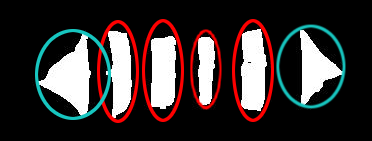
\includegraphics[width=.7\linewidth]{images/4}
    \caption{Partikelanalyse der Zwischenr\"aume der Ringe.}
    \label{fig:4}
\end{figure} 

Zu diesem Zeitpunkt k\"onnen  wir  mit  grosser  Sicherheit annehmen, dass die
meisten  Partikel,  die  noch \"ubriggeblieben sind, Widerstandsringe sind. Da
das Bild nicht unbedingt ausgerichtet aufgenommen wurde, muss die Orientierung
der Widerst\"ande  bestummen  werden. Dazu wird ausgenutzt, dass Widerst\"ande
(hoffentlich)   immer   \SI{90}{\degree}    zueinander    ausgerichtet   sind.

Die  Standardabweichungen  zum  Mittelwert  aller  Winkel  der Partikel werden
berechnet und die Outliers werden entfernt. Diese  Berechnung wird ein zweites
Mal durchgef\"uhrt mit  Winkel-Offsets von \SI{45}{\degree}. Der Grund daf\"ur
ist  weil  Partikel mit einer Orientierung nahe bei \SI{0}{\degree} wegen  dem
Wrap-Around  umherspringen,  was  aber  mit dem  Offset  nicht  passiert.  Die
Berechnung   mit  weniger  Outlier  wird  f\"ur  die   weiteren   Berechnungen
selektiert.

Die  Partikel  werden nach  ihrer  Orientierung  gefiltert,  sodass  nur  noch
Partikel mit $\SI{0}{\degree} \pm \SI{10}{\degree}$ oder $\SI{90}{\degree} \pm
\SI{10}{\degree}$ \"ubrig bleiben.

Aus der  kollektiven  Orientierung  der  \"ubrigbleibenden  Partikel  wird die
gesamte  Orientierung gewonnen und das Bild wird um diesen Winkel rotiert. Das
Resultat sieht nun wie in Abbildung \ref{fig:5} aus.

\begin{figure}[H]
    \centering
    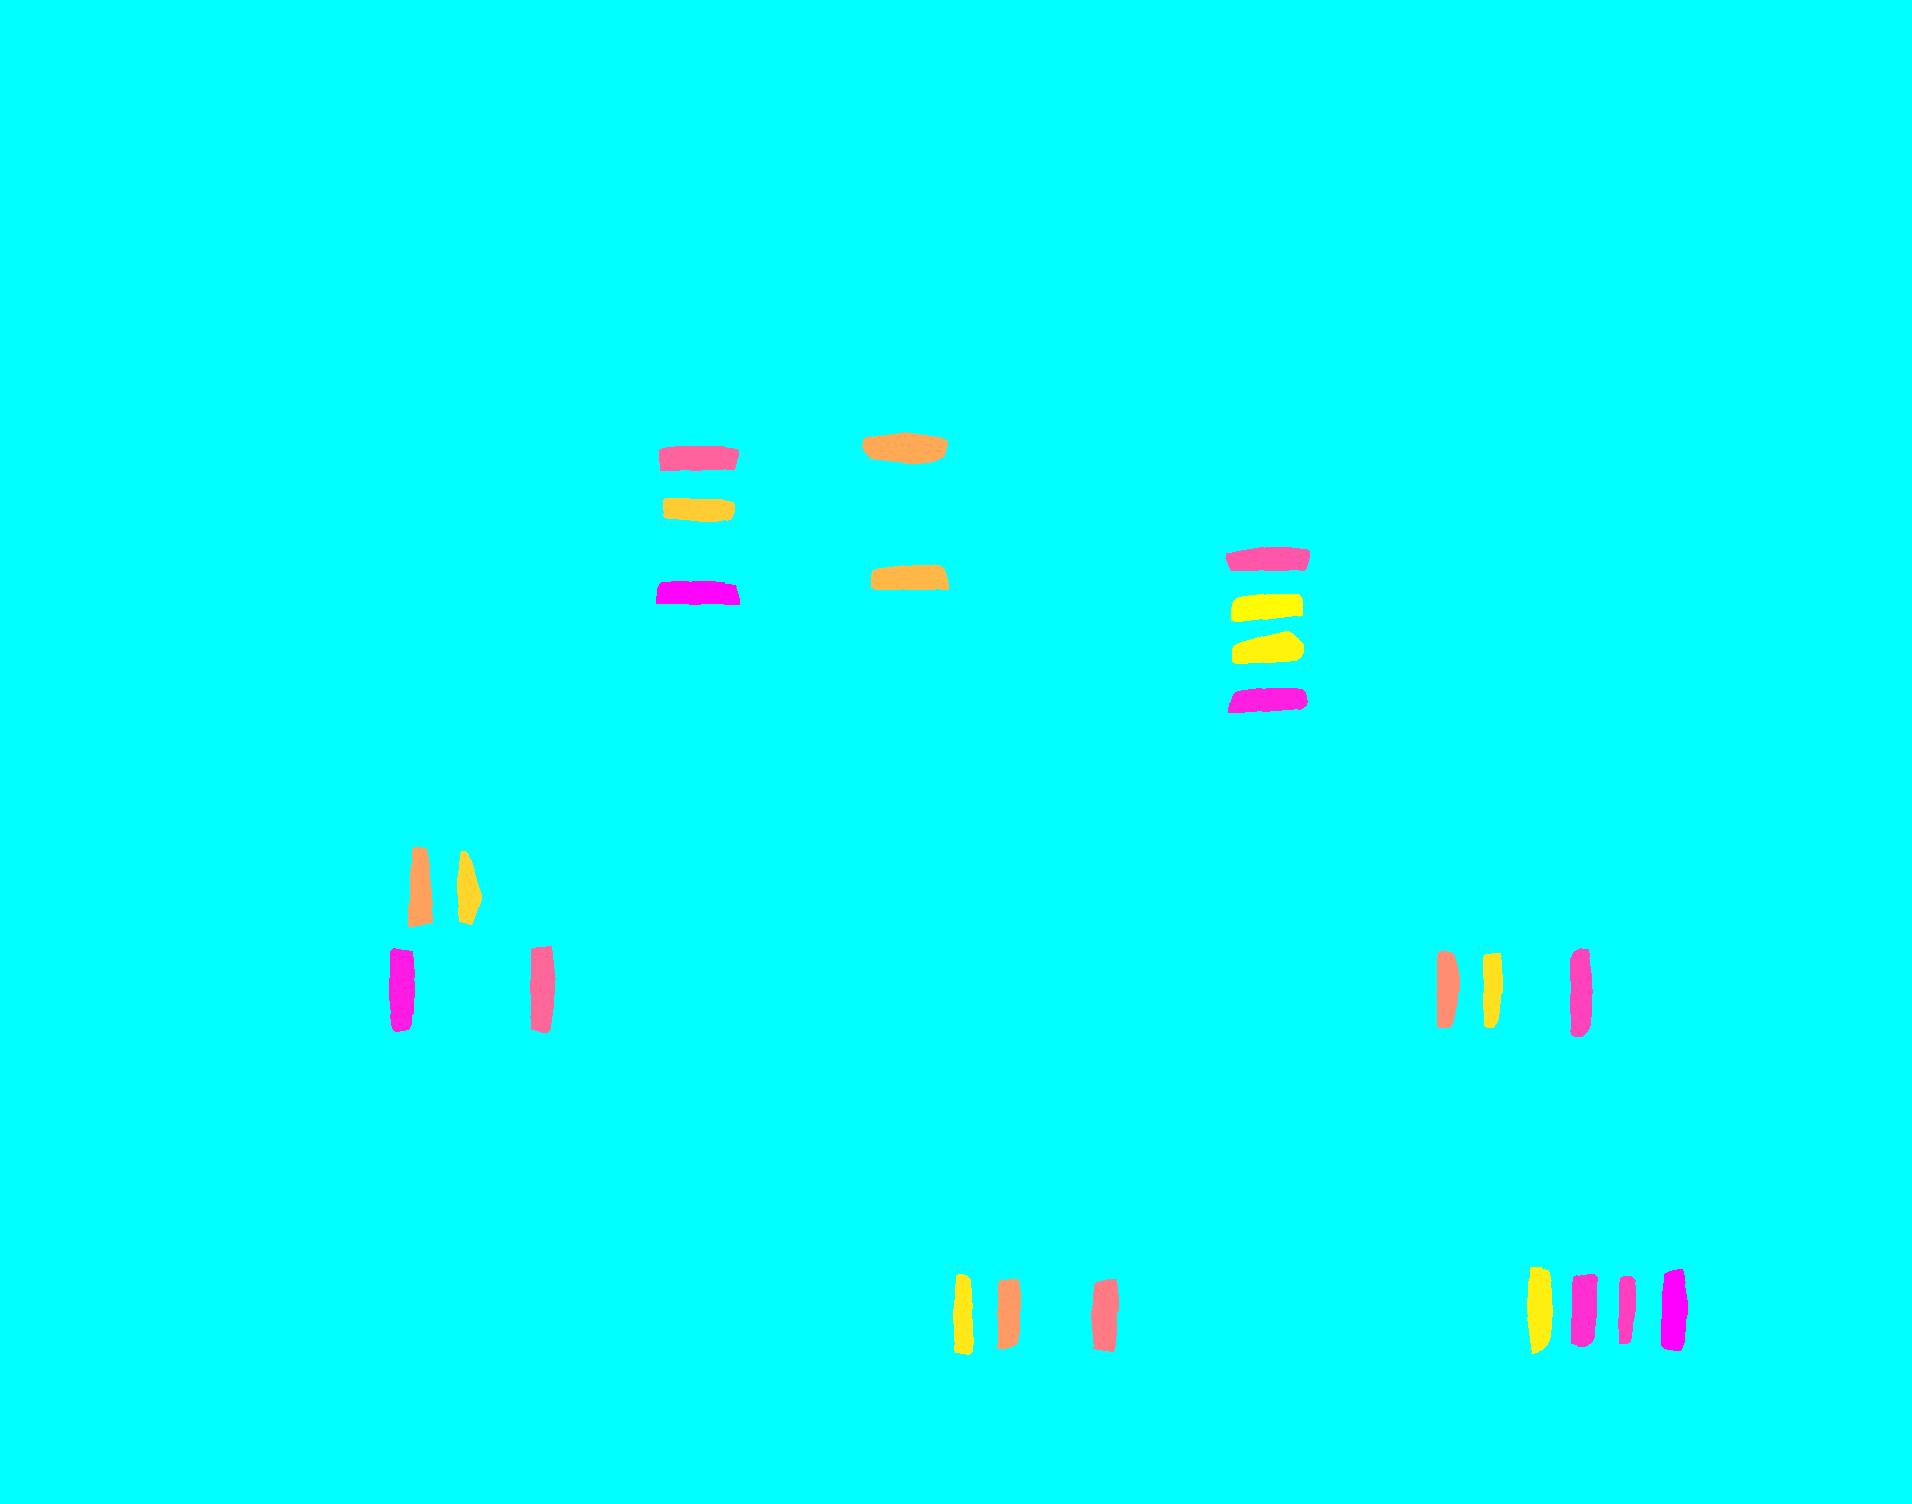
\includegraphics[width=.7\linewidth]{images/5}
    \caption{\"Ubrigbleigende Partikel nach der Winkelfilterung.}
    \label{fig:5}
\end{figure}

Die Partikel werden als n\"achstes stark verschmiert mit  einem  Gauss-Filter.
Die Filtergr\"osse  dabei  ist  exakt  die  Distanz  zwischen  zwei Ringe. Das
Resultat ist in der Abbildung \ref{fig:6} zu sehen.

\begin{figure}[H]
    \centering
    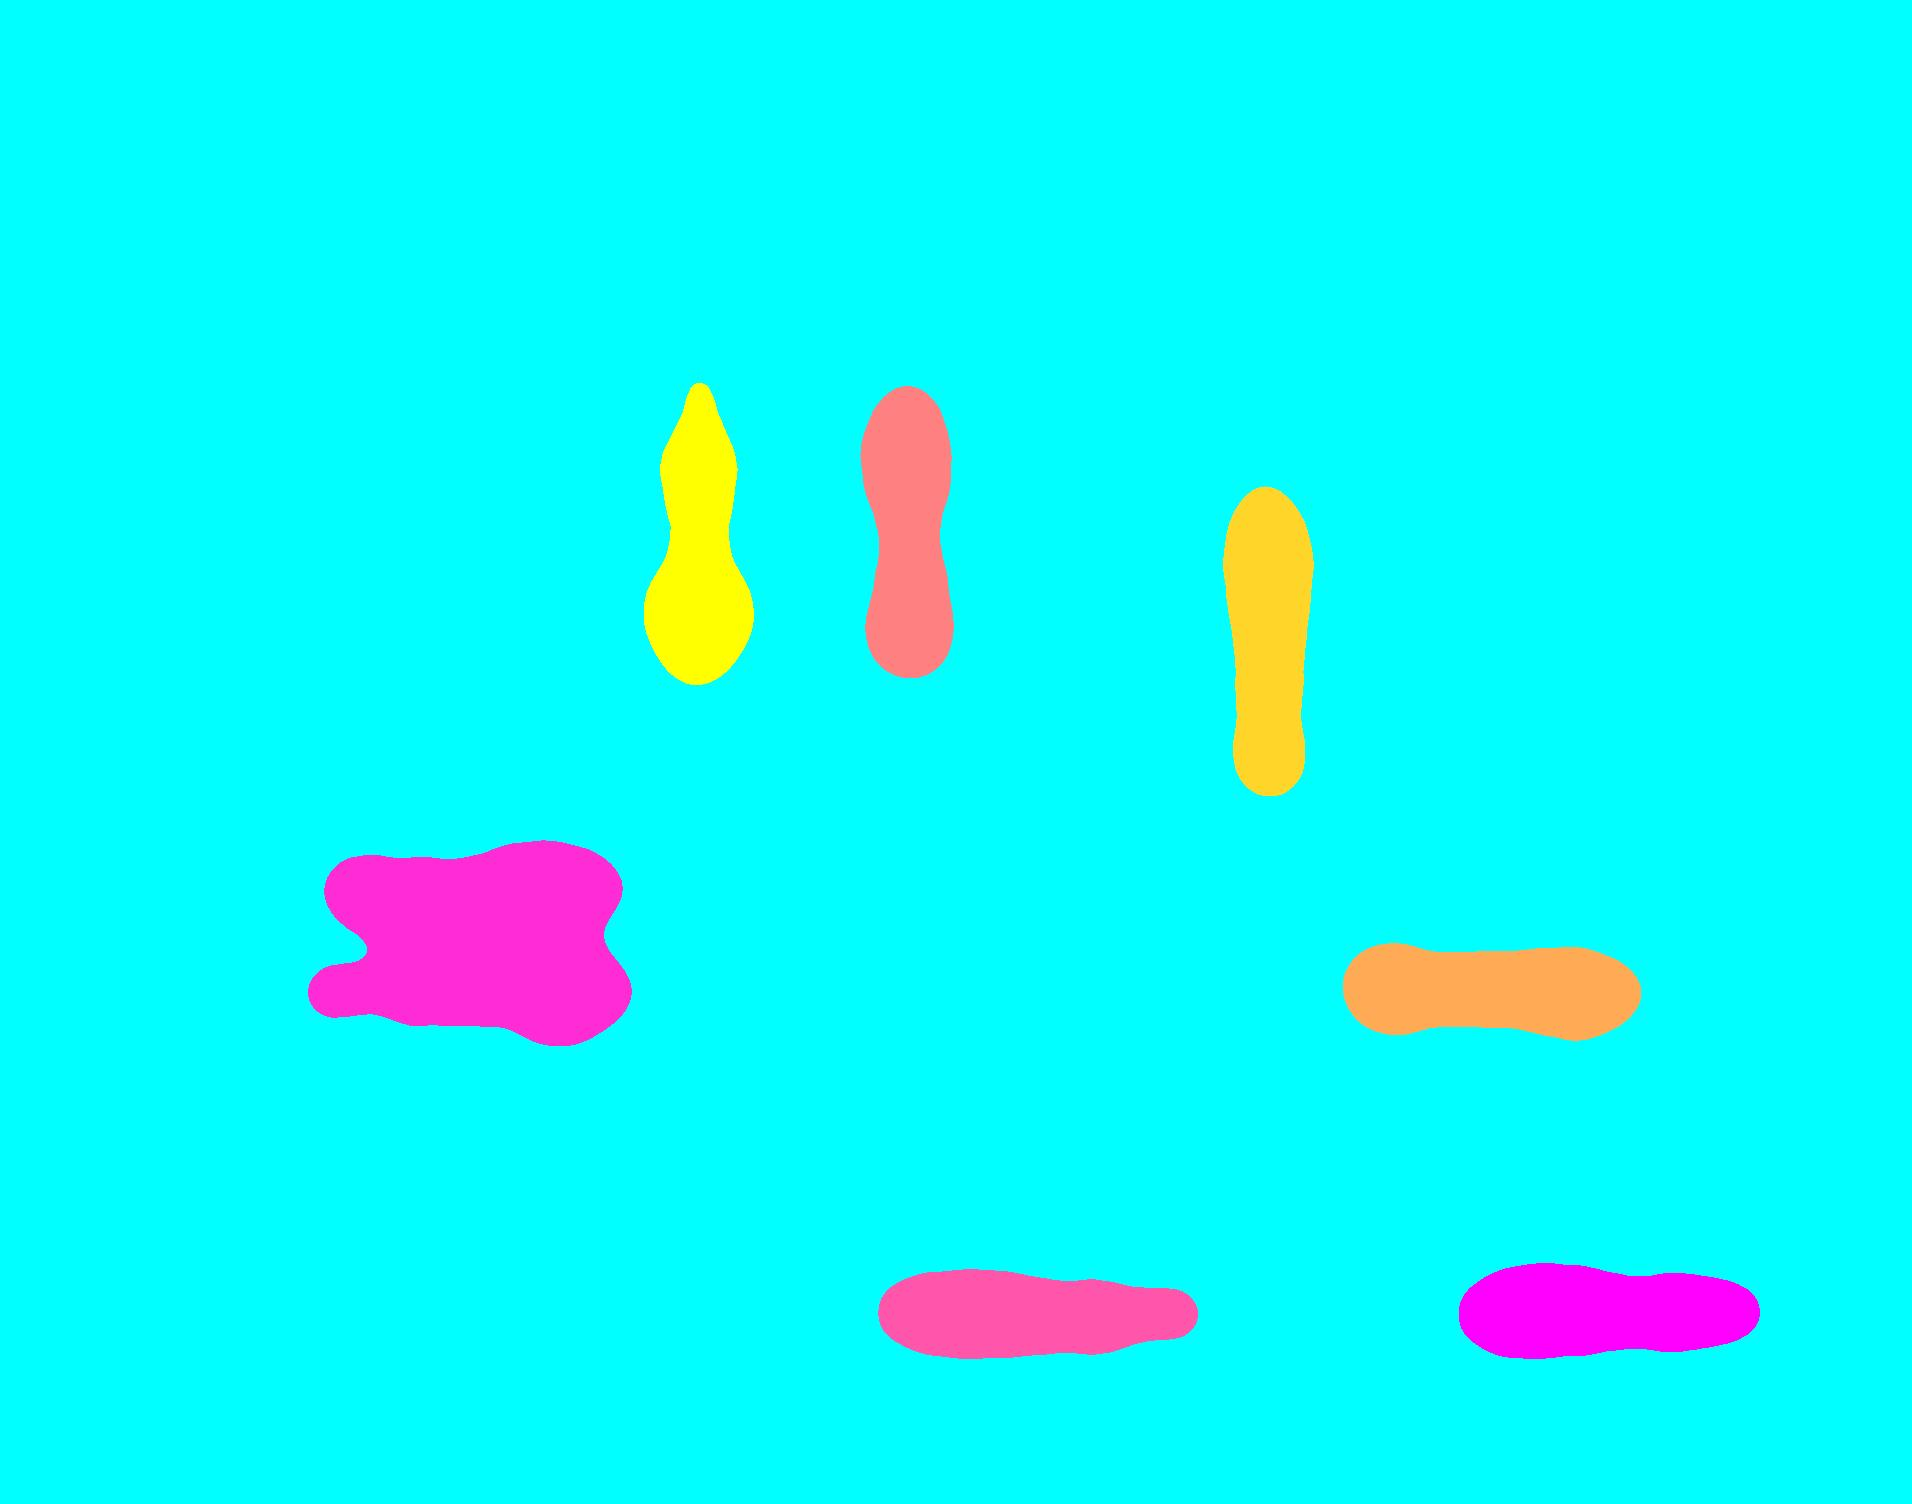
\includegraphics[width=.7\linewidth]{images/6}
    \caption{Verschmierung der Partikel f\"ur die Widerstandserkennung.}
    \label{fig:6}
\end{figure} 

Ein Problem das dabei auftritt  ist,  dass  Widerst\"ande,  die  nebeheinander
liegen, ineinander verschmieren. Um dieses Problem zu l\"osen kann  wieder die
Geometrie  eines  Widerstandes  ausgenutzt  werden.  Wenn  die  L\"ange  eines
Partikels nicht mindestens doppelt so lang ist wie  die Breite, so wird dieses
Partikel  in  der  Mitte  getrennt  (siehe  Abbildung  \ref{fig:7}).

\begin{figure}[H]
    \centering
    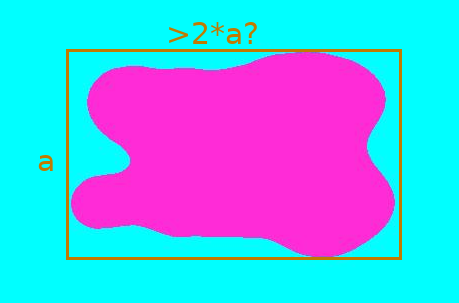
\includegraphics[width=.7\linewidth]{images/7}
    \caption{Trennung zwei ``verschmolzenen'' Widerst\"ande.}
    \label{fig:7}
\end{figure} 

Momentan  funktioniert  dieser  Ansatz  nur   f\"ur  zwei  Widerst\"ande,  die
nebeneinander  liegen. Bei drei oder mehr geht es  nicht,  aber  man  k\"onnte
einen  \"ahnlichen  Ansatz  verwenden  um  auch  dieses  Problem  zu  l\"osen.

Die neu gewonnenen Partikel \"uberdecken  jetzt  genau  die Widerst\"ande, die
wir  suchen.  Ein 1-pixel breiter Ausschnitt wird aus dem  Originalbild  f\"ur
jeden  Widerstand  extrahiert  (siehe  Abbildung  \ref{fig:8}), was f\"ur  die
Farberkennung verwendet wird.

\begin{figure}[H]
    \centering
    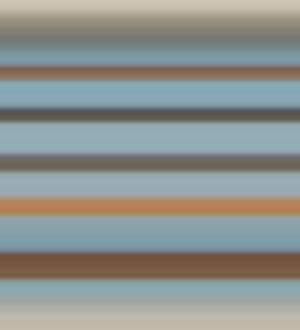
\includegraphics[width=.5\linewidth]{images/8}
    \caption{1-pixel breiter Ausschnitt eines Widerstandes.}
    \label{fig:8}
\end{figure}

